\documentclass[uplatex,dvipdfmx]{jsarticle}
\usepackage{ascmac}

\usepackage[uplatex,deluxe]{otf} % UTF
\usepackage[noalphabet]{pxchfon} % must be after otf package
\usepackage{stix2} % 欧文&数式フォント
\usepackage[fleqn,tbtags]{mathtools} % 数式関連 (w/ amsmath)
\usepackage{float} % フロートオプションH対応
\usepackage{listings,jvlisting}
\lstset{
  basicstyle={\ttfamily},
  identifierstyle={\small},
  commentstyle={\smallitshape},
  keywordstyle={\small\bfseries},
  ndkeywordstyle={\small},
  stringstyle={\small\ttfamily},
  frame={tb},
  breaklines=true,
  columns=[l]{fullflexible},
  numbers=left,
  xrightmargin=0zw,
  xleftmargin=3zw,
  numberstyle={\scriptsize},
  stepnumber=1,
  numbersep=1zw,
  lineskip=-0.5ex
}
\begin{document}

\title{仕様書} %システム名 仕様書 という形式にする
\author{24G1007 網中洲}
\date{2025年01月7日}
\maketitle

\section{概要}
このアプリケーションは,シンプルな掲示板(BBS)システムを実装している.ユーザーは以下の操作を行うことができる.
\begin{enumerate}
  \item 投稿(名前,メッセージの送信).
  \item 投稿一覧の取得(リアルタイム更新).
  \item 投稿の検索(キーワード検索).
  \item 投稿の編集および削除.
  \item 投稿への「いいね」.
\end{enumerate}

\section{利用者向けの説明}
画面のレイアウトは,以下の図\ref{reiauto}のようになる.
「送信」ボタンを押すと,名前とメッセージが送信され,「投稿チェック」ボタンを押すと,投稿された名前とメッセージを閲覧できる.
さらに,投稿されたメッセージごとに「いいね」ボタン,「編集」ボタン,「削除」ボタンがある.
これらは,投稿されたメッセージの評価,編集,削除ができる.
また,上部に「検索」ボタンがある.これは,検索したいメッセージの一部を入力することで,見たいメッセージを検索できる.

\begin{figure}[H]
  \centering
      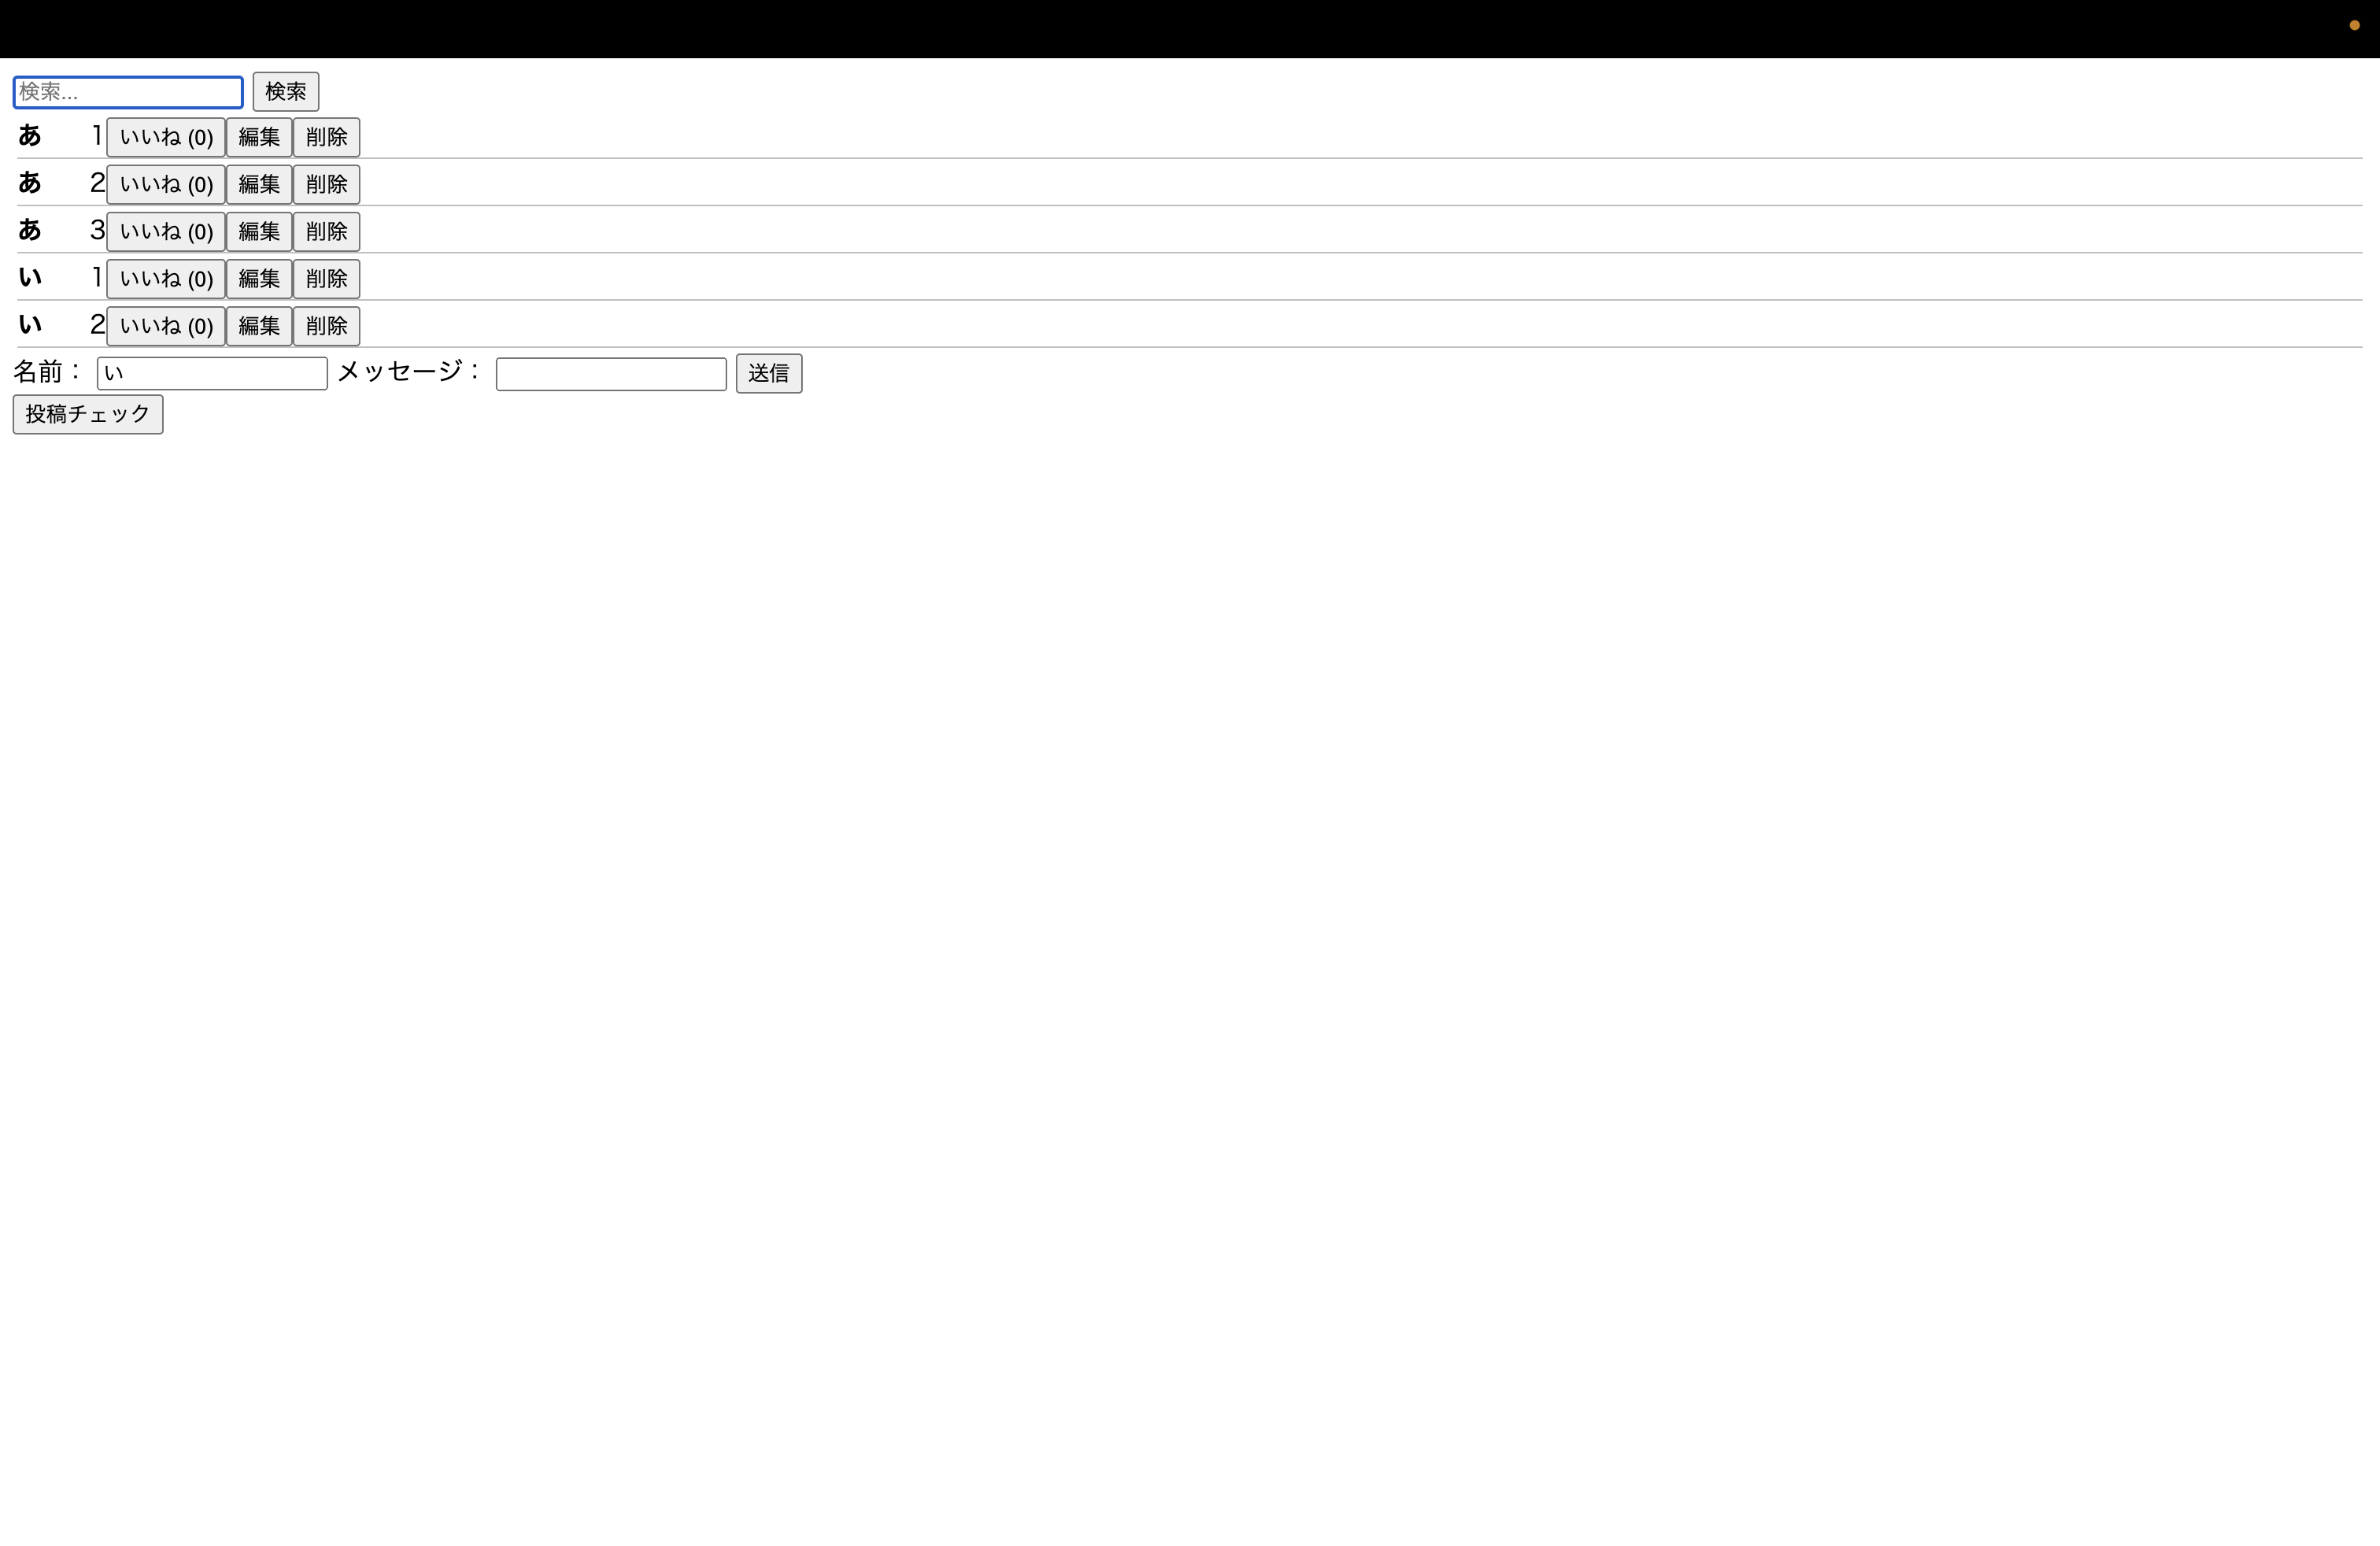
\includegraphics[width=15cm]{Figs/reiauto.png}
      \caption{画面のレイアウト}
      \label{reiauto}
\end{figure}

\section{管理者向けの説明}
このサーバーを立ち上げる手順以下のようになる.
\begin{enumerate}
  \item ターミナルを開き,`node app8.js` と入力(ホスト名は `localhost`,ポート番号は `8080`).
  \item 別のウィンドウでターミナルを開き,`telnet localhost 8080` と入力.
  \item WebブラウザのURL欄に `http://localhost:8080/public/bbs.html` と入力し,ページを表示する.
\end{enumerate}

\section{開発者向けの説明}
\subsection{サーバー側プログラムの構成と説明(app8.js)}
役割として,サーバーは,クライアントからのリクエストに応じて投稿データを操作し,レスポンスを返す.
主なエンドポイントは,投稿作成,一覧取得,いいね,検索,編集,削除などを提供する.
投稿データは bbs 配列に保存される(一時的なメモリ管理).また,図\ref{1}は,本システムのシーケンス図である.







\begin{figure}[H]
  \centering
      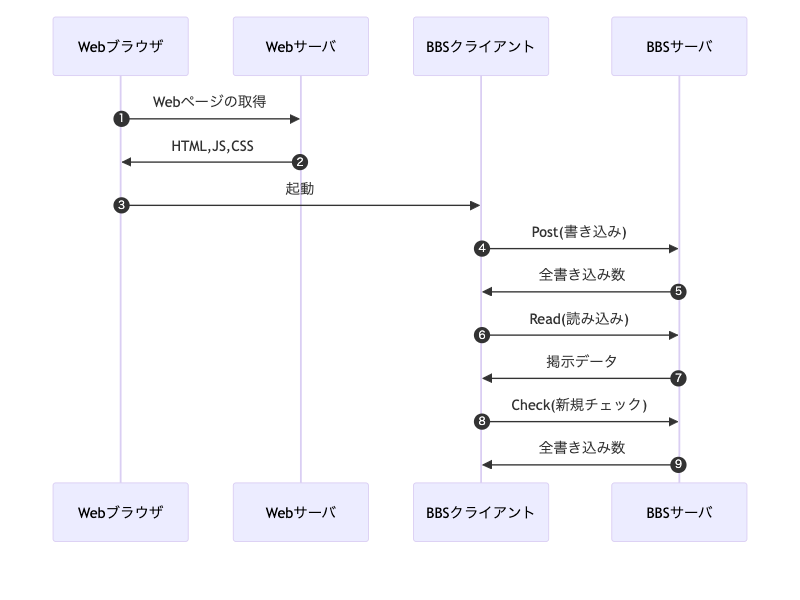
\includegraphics[width=15cm]{Figs/1.png}
      \caption{本システムのシーケンス図}
      \label{1}
\end{figure}


\subsubsection{初期設定}

\begin{lstlisting}[label=a]
const express = require("express");
const app = express();
app.use(express.urlencoded({ extended: true }));
app.use("/public", express.static(__dirname + "/public"));
\end{lstlisting}


\begin{itembox}[c]{プログラムの追加説明}
    \begin{enumerate}
        \setlength{\leftskip}{0pt}
        \item[・]expressはルーティングとリクエストの処理を簡略化する.
        \item[・]express.urlencodedはフォームデータを解析するミドルウェア.
    \end{enumerate}
\end{itembox}

\subsubsection{ 投稿データの管理}
\begin{lstlisting}[label=a]
let bbs = [];
\end{lstlisting}

\begin{itembox}[c]{プログラムの追加説明}
    \begin{enumerate}
        \setlength{\leftskip}{0pt}
        \item[・]投稿データをメモリ内で管理.
        \item[・]配列を簡易的なデータストアとして使用.
    \end{enumerate}
\end{itembox}

\subsubsection{投稿作成エンドポイント}
\begin{lstlisting}[label=b]
app.post("/post", (req, res) => {
  const name = req.body.name;
  const message = req.body.message;
  console.log([name, message]);
  bbs.push({ name: name, message: message, likes: 0 });
  res.json({ number: bbs.length });
});
\end{lstlisting}

\begin{itembox}[c]{処理内容}
    \begin{enumerate}
        \setlength{\leftskip}{0pt}
        \item[1]req.body から name と message を取得.
        \item[2]投稿データに初期値 { likes: 0 } を追加.
        \item[3]bbs 配列に保存.
        \item[4]新しい投稿数をレスポンスとして返却.
    \end{enumerate}
\end{itembox}

\subsubsection{投稿一覧取得エンドポイント}
\begin{lstlisting}[label=c]
app.post("/read", (req, res) => {
  const start = Number(req.body.start);
  const messages = start === 0 ? bbs : bbs.slice(start);
  res.json({ messages });
});

\end{lstlisting}

\begin{itembox}[c]{処理内容}
    \begin{enumerate}
        \setlength{\leftskip}{0pt}
        \item[1]start インデックスから投稿を取得.
        \item[2]投稿全体または一部をレスポンスとして返却.
    \end{enumerate}
\end{itembox}

\subsubsection{いいねエンドポイント}
\begin{lstlisting}[label=d]
app.post("/like", (req, res) => {
  const id = Number(req.body.id);
  if (id >= 0 && id < bbs.length) {
    bbs[id].likes = (bbs[id].likes || 0) + 1;
    res.json({ likes: bbs[id].likes });
  } else {
    res.status(400).json({ error: "Invalid ID" });
  }
});
\end{lstlisting}

\begin{itembox}[c]{処理内容}
    \begin{enumerate}
        \setlength{\leftskip}{0pt}
        \item[1]id に対応する投稿を検索.
        \item[2]該当する投稿の likes をインクリメント.
        \item[3]新しい「いいね」数を返却.
    \end{enumerate}
\end{itembox}

\subsubsection{検索エンドポイント}
\begin{lstlisting}[label=e]
app.post("/search", (req, res) => {
  const keyword = req.body.keyword.toLowerCase();
  const results = bbs.filter(
    (post) =>
      post.name.toLowerCase().includes(keyword) ||
      post.message.toLowerCase().includes(keyword)
  );
  res.json({ messages: results });
});
\end{lstlisting}

\begin{itembox}[c]{処理内容}
    \begin{enumerate}
        \setlength{\leftskip}{0pt}
        \item[1]キーワードで投稿をフィルタリング.
        \item[2]投稿者名またはメッセージにキーワードが含まれる投稿をレスポンスとして返却.
    \end{enumerate}
\end{itembox}


\subsubsection{ 編集エンドポイント}
\begin{lstlisting}[label=f]
app.put("/edit/:id", (req, res) => {
  const id = Number(req.params.id); // URL パラメータ ":id" を取得し数値に変換
  const newMessage = req.body.message; // リクエストボディから "message" を取得
  if (id >= 0 && id < bbs.length) { // ID が有効な範囲内か確認
    bbs[id].message = newMessage; // 投稿内容を新しいメッセージに更新
    res.json({ 
      success: true, 
      updatedMessage: bbs[id] // 更新後の投稿データを返却
    });
  } else {
    res.status(400).json({ error: "Invalid ID" }); // 無効な ID の場合エラーを返却
  }
});
\end{lstlisting}

\begin{itembox}[c]{処理内容}
    \begin{enumerate}
        \setlength{\leftskip}{0pt}
        \item[1]クライアントがリクエストした投稿の id(投稿の配列インデックス)を URL パラメータから取得.
        \item[2]クライアントがリクエストボディで送信した message を取得.
        \item[3]id が bbs 配列の範囲内(0 以上、bbs.length - 1 以下)かを確認.条件を満たさない場合、ステータスコード 400 とエラーメッセージを返却.
        \item[4]該当する投稿(bbs[id])の message を新しいメッセージで上書き
        \item[5]更新が成功した場合,success: true と更新後の投稿データ(bbs[id])を JSON 形式で返却
        \item[6]無効な id(例: 配列範囲外のインデックス)に対してエラーを返却
    \end{enumerate}
\end{itembox}


\subsubsection{ 削除エンドポイント}
\begin{lstlisting}[label=g]
app.delete("/delete/:id", (req, res) => {
  const id = Number(req.params.id); // URL パラメータ ":id" を取得し数値に変換
  if (id >= 0 && id < bbs.length) { // ID が有効な範囲内か確認
    bbs.splice(id, 1); // 指定された投稿を削除
    res.json({ success: true }); // 成功レスポンスを返却
  } else {
    res.status(400).json({ error: "Invalid ID" }); // 無効な ID の場合エラーを返却
  }
});
\end{lstlisting}

\begin{itembox}[c]{処理内容}
    \begin{enumerate}
        \setlength{\leftskip}{0pt}
        \item[1]クライアントがリクエストした投稿の id(投稿の配列インデックス)を URL パラメータから取得.
        \item[2]id が bbs 配列の範囲内(0 以上、bbs.length - 1 以下)かを確認.条件を満たさない場合、ステータスコード 400 とエラーメッセージを返却.
        \item[3]bbs.splice(id, 1) を使用して、該当する投稿を削除.splice は指定したインデックスの要素を削除し、配列を更新.
        \item[4]削除が成功した場合、success: true を JSON 形式で返却.
        \item[5]無効な id(例: 配列範囲外のインデックス)に対してエラーを返却
    \end{enumerate}
\end{itembox}


\subsection{クライアント側プログラムの構成と説明(bbs.js)}

\subsubsection{初期設定}

\begin{lstlisting}[label=h]
let number = 0;
const bbs = document.querySelector('#bbs');
\end{lstlisting}


\begin{itembox}[c]{プログラムの追加説明}
    \begin{enumerate}
        \setlength{\leftskip}{0pt}
        \item[・]numberはサーバーから取得した投稿数を追跡.
        \item[・]bbsは投稿を表示する HTML 要素.
    \end{enumerate}
\end{itembox}


\subsubsection{投稿送信処理}
\begin{lstlisting}[label=i]
document.querySelector('#post').addEventListener('click', () => {
  const name = document.querySelector('#name').value;
  const message = document.querySelector('#message').value;
  const params = new URLSearchParams({ name, message });
  fetch("/post", {
    method: "POST",
    body: params,
    headers: { 'Content-Type': 'application/x-www-form-urlencoded' }
  })
  .then((response) => response.json())
  .then(() => {
    document.querySelector('#message').value = "";
  });
});
\end{lstlisting}

\begin{itembox}[c]{処理内容}
    \begin{enumerate}
        \setlength{\leftskip}{0pt}
        \item[1]フォーム入力値を取得.
        \item[2]fetch を使用してサーバーに非同期リクエストを送信.
        \item[3]レスポンスを受け取った後、入力フィールドをクリア.
    \end{enumerate}
\end{itembox}


\subsubsection{投稿一覧の取得}
\begin{lstlisting}[label=j]
document.querySelector('#check').addEventListener('click', () => {
  fetch("/check", { method: "POST" })
  .then((response) => response.json())
  .then((response) => {
    if (number != response.number) {
      fetch("/read", {
        method: "POST",
        body: `start=${number}`,
        headers: { 'Content-Type': 'application/x-www-form-urlencoded' }
      })
      .then((response) => response.json())
      .then((response) => {
        number += response.messages.length;
        response.messages.forEach((mes) => {
          const cover = document.createElement('div');
          cover.className = 'cover';
          cover.innerHTML = `
            <span class="name">${mes.name}</span>
            <span class="mes">${mes.message}</span>
          `;
          bbs.appendChild(cover);
        });
      });
    }
  });
});
\end{lstlisting}

\begin{itembox}[c]{処理内容}
    \begin{enumerate}
        \setlength{\leftskip}{0pt}
        \item[1]サーバーに現在の投稿数を問い合わせ.
        \item[2]新しい投稿があれば、それを取得して画面に追加表示.
    \end{enumerate}
\end{itembox}

\subsubsection{いいね操作}
\begin{lstlisting}[label=k]
let like_button = document.createElement('button');
like_button.innerText = `いいね (${mes.likes || 0})`;
like_button.addEventListener('click', () => {
  fetch('/like', {
    method: "POST",
    body: `id=${mes.id}`,
    headers: { 'Content-Type': 'application/x-www-form-urlencoded' }
  })
  .then((response) => response.json())
  .then((data) => {
    like_button.innerText = `いいね (${data.likes})`;
  });
});
\end{lstlisting}

\begin{itembox}[c]{処理内容}
    \begin{enumerate}
        \setlength{\leftskip}{0pt}
        \item[1]ボタンを動的に生成し,現在の「いいね」数を表示するテキストを設定.
        \item[2]ボタンがクリックされたとき,サーバーに対象投稿の「いいね」操作をリクエスト.
        \item[3]/like エンドポイントに POST リクエストを送信.リクエストには投稿 ID を含むデータを送る.
        \item[4]サーバーから新しい「いいね」数を受け取り,ボタンの表示を更新
    \end{enumerate}
\end{itembox}


\end{document}










